\documentclass[a4paper, 12 pt, conference]{ieeeconf}  % 
\IEEEoverridecommandlockouts                              % This command is only
% needed if you want to
% use the \thanks command

\overrideIEEEmargins
% See the \addtolength command later in the file to balance the column lengths
% on the last page of the document

% Pacote de acentuação
\usepackage[brazil]{babel}
\usepackage[utf8]{inputenc}

% The following packages can be found on http:\\www.ctan.org
\usepackage{graphics} % for pdf, bitmapped graphics files
\usepackage{epsfig} % for postscript graphics files
%\usepackage{mathptmx} % assumes new font selection scheme installed
%\usepackage{mathptmx} % assumes new font selection scheme installed
\usepackage{amsmath} % assumes amsmath package installed
\usepackage{amssymb}  % assumes amsmath package installed

\usepackage[]{todonotes} % adicionar parâmetro [disable] para ocultar os comentários
\usepackage{xspace} % usado nos comentários
\usepackage[normalem]{ulem}

\newcounter{todocounter}
\setlength{\marginparwidth}{2cm}
\reversemarginpar
\newcommand{\nota}[1]{\xspace\stepcounter{todocounter}\todo[fancyline]{\thetodocounter: #1}}
\newcommand{\notain}[2]{\stepcounter{todocounter}\todo[inline]{\thetodocounter: (#1) #2}}

\title{\LARGE \bf
Relatório das práticas de aprendizado de máquina.
}

\author{Marcus V. S. Maziero$^{1}$, Paulo R. K. Nakaima$^{2}$, Vitor Hugo Borges Basseto$^{3}$% <-this % stops a space
\thanks{$^{1}$Marcus V. S. Maziero, $^{2}$Paulo R. K. Nakaima e $^{3}$Vitor Hugo Borges Basseto estão vinculados à Universidade Tecnológica Federal do Paraná, Av. Alberto Carazzai, 1640, Cornélio Procópio, Brasil. 
        {\tt\small marcus.maziero$@$outlook.com, nakaima$@$alunos.utfpr.edu.br, vitorhugobasseto$@$gmail.com}}%
}


\begin{document}


\maketitle
\thispagestyle{empty}
\pagestyle{empty}


%%%%%%%%%%%%%%%%%%%%%%%%%%%%%%%%%%%%%%%%%%%%%%%%%%%%%%%%%%%%%%%%%%%%%%%%%%%%%%%%
%%%%%%%%%%%%%%%%%%%%%%%%%%%%%%%%%%%%%%%%%%%%%%%%%%%%%%%%%%%%%%%%%%%%%%%%%%%%%%%%
\begin{abstract}
	Este relatório apresenta os resultado encontrados em 5 práticas de aprendizado de máquinas para classificação de imagens, mais especificamente, classificação de emoções com base em expressões faciais. A partir da Seção~\ref{pratica02} no final de cada uma das seções encontram-se os \textit{links} para o código fonte para desenvolvimento e exibição, sendo que o último possibilita ao leitor a execução imediata dos experimentos em qualquer navegador moderno.
\end{abstract}

\begin{keywords}
	Inteligencia Artificial, Emoções, Imagens, Machine Learning.
\end{keywords}


%%%%%%%%%%%%%%%%%%%%%%%%%%%%%%%%%%%%%%%%%%%%%%%%%%%%%%%%%%%%%%%%%%%%%%%%%%%%%%%%
%
%A Tabela \ref{Tabela_Exemplo} mostra um exemplo para inserir tabelas nesse documento e a Figura \ref{Figura_Exemplo} mostra um exemplo para inserir figuras nesse documento \cite{Buerger1989}.
%
%\begin{table}[!htbp]
%    \caption{Table Type Styles}
%    \begin{center}
%        \begin{tabular}{|c|c|c|c|}
%            \hline
%            \textbf{Table}&\multicolumn{3}{|c|}{\textbf{Table Column Head}} \\
%            \cline{2-4} 
%            \textbf{Head} & \textbf{\textit{Table column subhead}}& \textbf{\textit{Subhead}}& \textbf{\textit{Subhead}} \\
%            \hline
%            copy& More table copy$^{\mathrm{a}}$& &  \\
%            \hline
%        \end{tabular}
%    \label{Tabela_Exemplo}
%    \end{center}
%\end{table}
%
%\begin{figure}[!htbp]
%    \centering
%    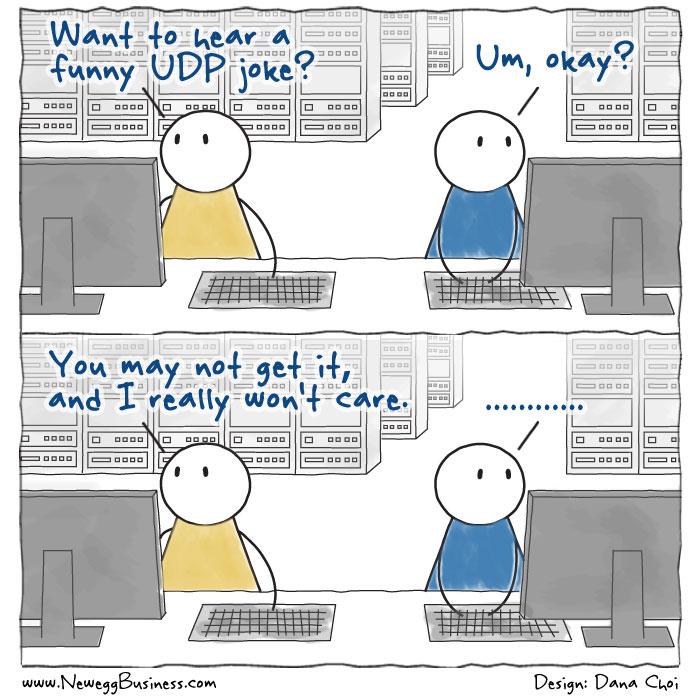
\includegraphics[width=0.8\linewidth,clip=true,trim=0cm 0cm 0cm 0cm, keepaspectratio=true]{Figura_Exemplo.png}
%    \caption{Example of a figure caption.}
%    \label{Figura_Exemplo}
%\end{figure}
%
%É importante também adicionar citações ao longo do texto para mostrar fundamentações, afirmações e trabalhos relacionados. Mais infomações sobre a adição de referências podem ser encontradas em \cite{BibTeX2014}.

\section{INTRODUÇÃO}
As práticas de aprendizado de maquina ou Machine Learning (ML) em inglês, é uma das maneiras de utilizar Inteligência Artificial (IA) para aprimorar o conhecimento de aplicações por técnicas de treinamento, proporcionando um aprendizado mais natural para a máquina.

O aprendizado de máquina consiste em promover para a aplicação experiências com diversos cenários para que o mesma após determinado tempo e quantidade de cenários aprenda e modifique seu comportamento.

Existem diversas empresas que já utilizam da aprendizagem de máquina conforme apresenta \cite{ray:2019}, para alcançar resultados benéficos em suas organizações, entre elas: Facebook, Google, Uber e Apple. Em algumas dessas empresas o ML é utilizado para recomendações de produtos e análise de tráfego.

Neste contexto foi realizado esse relatório com a proposta de demonstrar os resultados alcançados por intermédio de práticas propostas sobre o aprendizado de máquina.
\section{OBJETIVO}
Demonstrar os resultados alcançados após realizar as práticas propostas com bases de dados e técnicas de prática diversas.
\section{DEEP LEARNING}
O Aprendizado Profundo em inglês Deep Learning (DL) estão ligados à classificação de dados na utilização do Machine Learning.

O DL auxilia diversas aplicações com a classificação de dados, e assim gerando informações e tomadas de decisões mais claras pela máquina, isso acontece pois conforme \cite{ponti:2017}, o DL oferece um bloco de técnicas para analise de materiais visuais, com variados modelos e algoritmos.

Sendo assim ao utilizar do Deep Learning a proposta é aumentar a precisão dos dados, \cite{karatekin:2019} demonstra como a clareza de dados com DL pode ser usado no campo da medicina.

A falta de precisão nos dados coletados pode ocasionar em uma interpretação errada pela aplicação com Machihne Learning. Dessa forma a utilização do Deep Learning é importante no processo de aprendizado de máquina

\section{PRÁTICA 01}
\label{pratica01}
Nesta prática busca-se selecionar as bases de imagens, os descritores para extração de características e os classificadores.

\subsection{Base de dados}
Foi selecionada a base de imagens CKPLUS. A qual pode ser encontrada em: https://www.kaggle.com/shawon10/ckplus. Contém 981 imagens de rostos em escalas de cinza com as expressões de raiva, nojo, desprezo, medo, felicidade, tristeza, surpresa. Para este trabalho foram selecionadas apenas as expressões raiva, medo, felicidade, tristeza e surpresa.

A segunda base de imagens selecionada foi a Yale Face Database. A qual pode ser encontrada em: http://vision.ucsd.edu/content/yale-face-database. Contém 165 imagens em tons de cinza de rostos de 15 indivíduos fazendo 6 expressões faciais, normal, tristeza, sonolência, surpresa e piscando.

\subsection{Extração de características}
Para extração de características foi utilizado os descritores Local Binary Patterns (LBP) e o Gabor. Sendo que o primeiro extrai 256 caracterísitcas de textura é não paramétrico, possui baixo custo de processamento \cite{rajan:19}. Seu funcionamento consiste em dividir a imagem em sub-blocos sendo que para cada sub-bloco é calculado o histograma, o vetor de características é formado com a concatenação desses histogramas \cite{rajan:19}. O descritor Gabor extrai 60 características de textura como linhas e contornos. Os arquivos finais podem ser encontrados em: https://drive.google.com/drive/folders/1ZP-CkuoP2mQggsR2sd9QGcbks1hrt68u?usp=sharing.

\subsection{Seleção dos classificadores}
Os classificadores utilizados nas práticas seguintes foram selecionados com base em \cite{rajan:19}. Os classificadores são Regressão Logística (Logistic Regression - LR), K vizinhos mais próximos (k-nearest neighbors - KNN), Máquina de Vetores Suporte (Support Vectors Machine - SVM), rede perceptron multicamadas (Multi-layer Perceptron - MLP).

\section{PRÁTICA 02}
\label{pratica02}
Nesta prática busca-se comparar a acurácia obtida por diferentes classificadores a partir dos arquivos gerados na Seção~\ref{pratica01}.

\subsection{Descritor LBP}
\subsubsection{Seleção da técnica de normalização}
A partir dos arquivos gerados com os descritores foram alterandas as técnicas de normalizações para verificar qual delas atinge melhor resultado para acurácia. Para a base de dados CKPLUS com o descritor LBP as diferenças são mínimas como podem ser vistas na Figura~\ref{fig:bar_norm_all_lbp}. Os classificadores utilizados foram: LR, KNN, SVM, MLP.

\begin{figure}[!htbp]
	\centering
	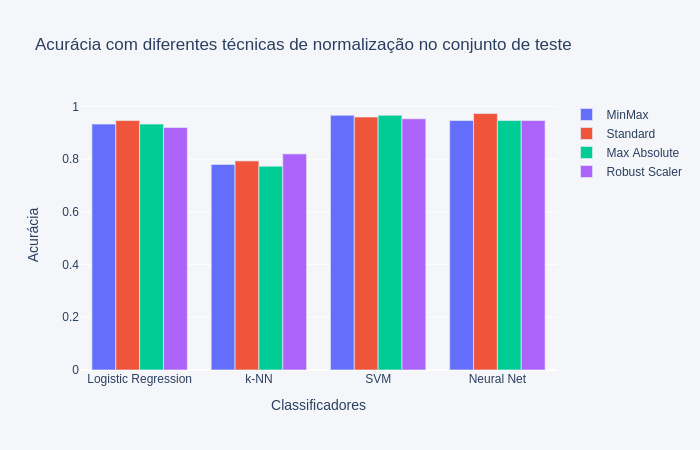
\includegraphics[width=1.0\linewidth,clip=true,trim=0cm 0cm 0cm 0cm, keepaspectratio=true]{bar_norm_all_lbp.png}
	\caption{Comparação de técnicas de normalização com descritor LBP.}
	\label{fig:bar_norm_all_lbp}
\end{figure}

O classificador MLP com a normalização Standard foi a que obteve o melhor resultado, 97\% de acurácia. O pior resultado foi obtido pelo classificador KNN com a normalização Max Absolute, 77\%.

\subsection{Descritor Gabor}
Para o descritor Gabor as diferenças entre os resultados obtidos foi alta para o classificador KNN, contudo nenhum dos classificadores obtiveram 50\% de acurácia. A técnica de normalização Min-Max que consiste em transformar cada característica com valor mínimo em 0 e os valores máximos em 1, sendo que o restando é tranformado em um valor decima entre 0 e 1, obteve a melhor acurácia com o classificador KNN, 41\%. O pior desempenho foi obtido pelo classificador KNN com a normalização Standard, 21\%. Os resultados podem ser vistos na Figura~\ref{fig:bar_norm_all_gabor} Foram mantidos os classificadores utilizados no último experimento.

\begin{figure}[!htbp]
	\centering
	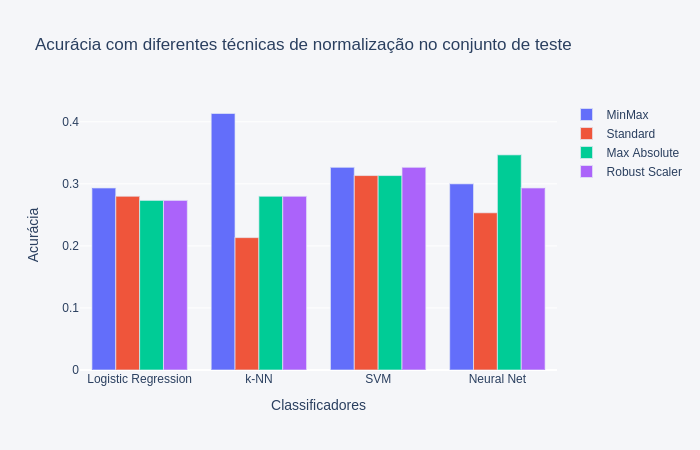
\includegraphics[width=1.0\linewidth,clip=true,trim=0cm 0cm 0cm 0cm, keepaspectratio=true]{bar_norm_all_gabor.png}
	\caption{Comparação de técnicas de normalização com descritor Gabor.}
	\label{fig:bar_norm_all_gabor}
\end{figure}

\subsubsection{Desenvolvimento} Prática 02 - ckplus  - LBP - all - norm; Prática 02 - ckplus  - Gabor - all - norm
\subsubsection{Exibição e Execução} ATUALIZAR

\section{PRÁTICA 03}
\label{pratica03}

Neste experimento busca-se utilizar aprendizado não supervisionado com o classificador \textit{k-means} de modo a obter o melhor valor de \textit{k}. Além disto busca-se reduzir a dimensão do conjunto de dados de modo a reter 90\% de variância.

\subsection{Descritor LBP}
\subsubsection{Redução de dimensionalidade}

Buscou-se reduzir a dimensionalidade do conjunto de dados obtidos com o descritor LBP de modo a reter 90\% de variância. Primeiramente os dados foram normalizados com a técnica Standard, ou seja, são calculados a média e o desvio padrão da conjunto de amostras, em seguida é subraída de cada amostra a média, o resultado então é divido pelo desvio padrão. Esta técnica foi selecionada pois obteve resultado levemente superior as outras técnicas na Seção~\ref{pratica02}.

Com a técnica PCA para redução de dimensionalidade foi selecionado o menor número de componentes que retinha 90\% de variância. Ver Figura~\ref{fig:points_pca_lbp}. Foi possível reduzir de 256 para 133 característica.

\begin{figure}[!htbp]
	\centering
	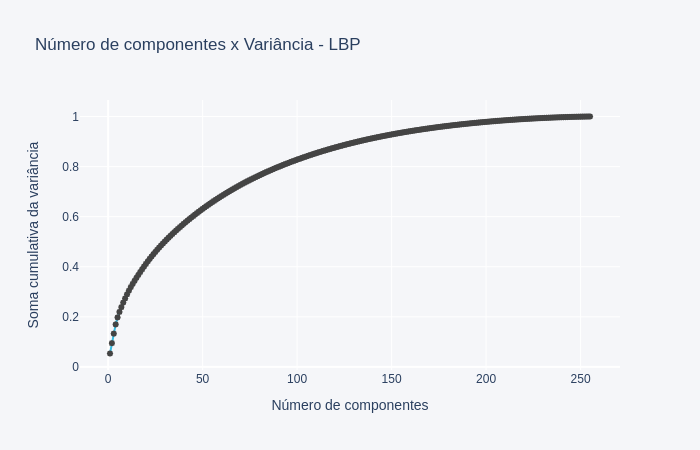
\includegraphics[width=1.0\linewidth,clip=true,trim=0cm 0cm 0cm 0cm, keepaspectratio=true]{points_pca_lbp.png}
	\caption{Selecionar o menor número de componentes retendo 90\% de variância.}
	\label{fig:points_pca_lbp}
\end{figure}

\subsubsection{Agrupamento}
Com a redução de dimensionalidade obtida foi utilizado o classificador k-means agrupando as amostras de 2 a 30 agrupamentos de forma iterativa. Ao fim, foi compilado e plotado a variância para cada quantidade de agrupamentos para aplicar o método elbow com intuito de definir a melhor quantidade de agrupamentos. O ponto mais distante da reta formada pela ligação do ponto inicial ao final foi 9, o melhor número de agrupamentos. Ver Figura~\ref{fig:points_elbow_lbp}. O agrupamento final foi plotado destancando-se os centróides na Figura~\ref{fig:scatter_k9_lbp}.

\begin{figure}[!htbp]
	\centering
	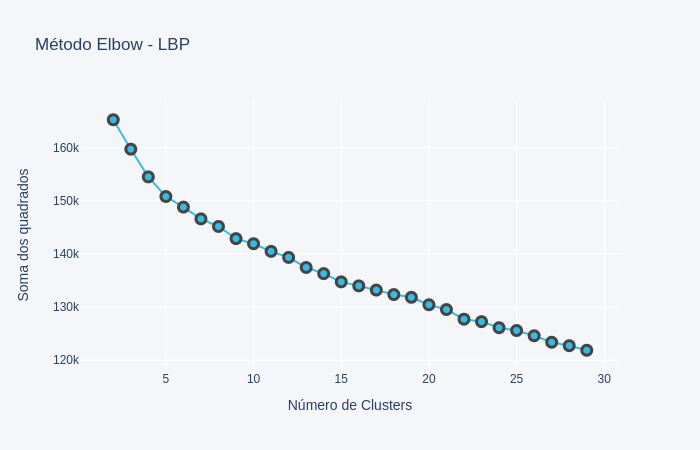
\includegraphics[width=1.0\linewidth,clip=true,trim=0cm 0cm 0cm 0cm, keepaspectratio=true]{points_elbow_lbp.png}
	\caption{Selecionar o melhor número de agrupamentos.}
	\label{fig:points_elbow_lbp}
\end{figure}

\begin{figure}[!htbp]
	\centering
	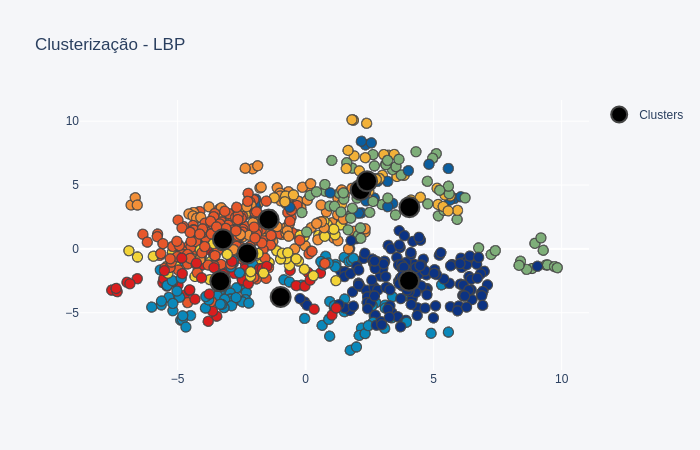
\includegraphics[width=1.0\linewidth,clip=true,trim=0cm 0cm 0cm 0cm, keepaspectratio=true]{scatter_k9_lbp.png}
	\caption{Conjuto de amostras agrupados em 9.}
	\label{fig:scatter_k9_lbp}
\end{figure}

\subsection{Descritor Gabor}
\subsubsection{Redução de dimensionalidade}
Foi aplicada a técnica PCA para as características extraídas com o descritor Gabor. Primeiramente os dados  foram normalizados com a técnica MinMax, melhor resultado obtido no experimento anterior. Foi possível reduzir as características de 60 para duas retendo 100\% de variância. Ver  Figura~\ref{fig:points_pca_gabor}.

\begin{figure}[!htbp]
	\centering
	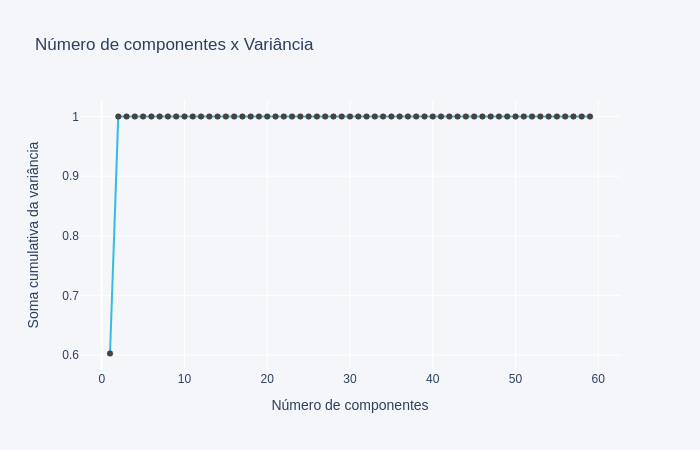
\includegraphics[width=1.0\linewidth,clip=true,trim=0cm 0cm 0cm 0cm, keepaspectratio=true]{points_pca_gabor.png}
	\caption{Selecionar o menor número de componentes retendo 100\% de variância.}
	\label{fig:points_pca_gabor}
\end{figure}

\subsubsection{Agrupamento}
Na sequência foi utilizado o classificador k-means agrupando as amostras de 2 a 30 agrupamentos de forma iterativa. Ao fim, foi compilado e plotado a variância para cada quantidade de agrupamentos para aplicar o método elbow com intuito de definir a melhor quantidade de agrupamentos. O ponto mais distante da reta formada pela ligação do ponto inicial ao final foi 8, o melhor número de agrupamentos. Ver Figura~\ref{fig:points_elbow_gabor}. O agrupamento final foi plotado destancando-se os centróides na Figura~\ref{fig:scatter_k8_gabor}.

\begin{figure}[!htbp]
	\centering
	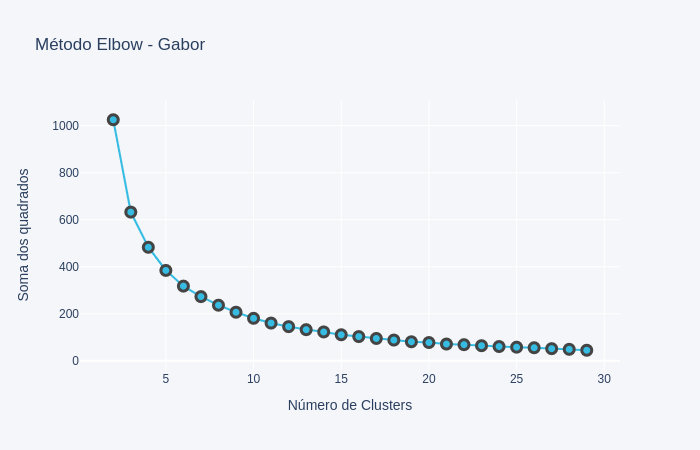
\includegraphics[width=1.0\linewidth,clip=true,trim=0cm 0cm 0cm 0cm, keepaspectratio=true]{points_elbow_gabor.png}
	\caption{Selecionar o melhor número de agrupamentos.}
	\label{fig:points_elbow_gabor}
\end{figure}

\begin{figure}[!htbp]
	\centering
	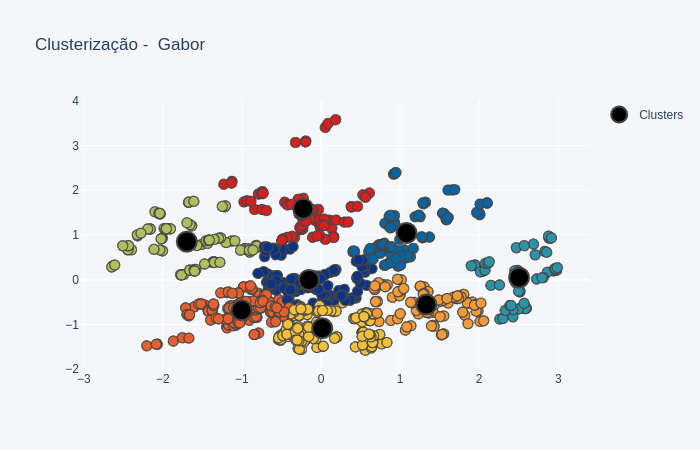
\includegraphics[width=1.0\linewidth,clip=true,trim=0cm 0cm 0cm 0cm, keepaspectratio=true]{scatter_k8_gabor.png}
	\caption{Conjuto de amostras agrupados em 8.}
	\label{fig:scatter_k8_gabor}
\end{figure}

Nota-se que o agrupamento plotado na Figura~\ref{fig:scatter_k8_gabor} possui fronteiras mais definidas do que na Figura~\ref{fig:scatter_k9_lbp}.

\subsubsection{Desenvolvimento} Prática 03 - ckplus - LBP - pca - kmeans; Prática 03 - ckplus - Gabor - pca - kmeans
\subsubsection{Exibição e Execução} ATUALIZAR

\section{PRÁTICA 04}
\label{pratica04}
Nesta prática busca-se comparar os resultados de aprendizado supervisionado realizado nos experimentos anteriores com o método Label Propagation.

\subsection{Descritor LBP}
\subsubsection{Seleção dos parâmetros para o método Label Propagation}
O método Label Propagation pode ser utilizado com o kernel de k vizinhos mais próximos (K-Nearest Neighbors - KNN) e funçao de base radial (Radial Basis Function - RBF). Para o  primeiro caso deve-se definir o número máximo de iterações o número de vizinhos e outros. Para o RBF deve-se definir o valor gamma, a quantidade máxima de iterações e outros.

Para este experimento variou-se o kernel entre KNN e RBF, o valor gama em 20, 25, 30, a quantidade máxima de iterações em 300, 500, 1000 e o número de vizinhos em 7, 14, 21 e 28. Para cada combinação foi feita a validação cruzada em 5 partições. O critério para definição dos melhores parâmetros foi a média da acurácia. Os melhores parâmetros para o kernel KNN e RBF estão descritos na Tabela~\ref{tab:meida_acuracia_lp_lbp}. Para todos os classificadores o desempenho da acurácia apresentou queda quando comparado as técnincas supervisionadas. Contudo existe a redução de 600 imagens rotuladas para 360. A comparação com os resultados das práticas supervisionadas podem ser vistas na Figura~\ref{fig:super_vs_semi_lbp}.


\begin{table}[!htbp]
    \caption{Média e desvio padrão para acurácia}
    \begin{center}
        \begin{tabular}{lllllll}
        	Kernel & Iteração & Vizinhos & Gamma &  Média & Desv. Pad. & Pos. \\
        	\hline
        	KNN    & 300             & 7                  & n/a  & 0.39       & 0.021               & 1       \\
        	\hline
        	RBF    & 300             & n/a                & 20   & 0.10       & 0.003               & 13      \\
        \end{tabular}
    \label{tab:meida_acuracia_lp_lbp}
    \end{center}
\end{table}

\begin{figure}[!htbp]
	\centering
	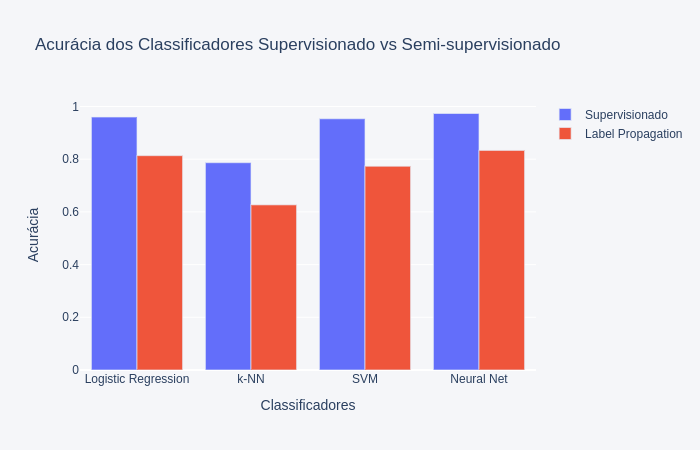
\includegraphics[width=1.0\linewidth,clip=true,trim=0cm 0cm 0cm 0cm, keepaspectratio=true]{bar_supervisionado_vs_semi_lbp.png}
	\caption{Supervisionado vs Semi-supervisionado.}
	\label{fig:super_vs_semi_lbp}
\end{figure}

\subsubsection{Desenvolvimento} Prática 02 - ckplus  - LBP - standard; Prática 04 - ckpuls - LBP - gridsearch - both; Prática 04 - ckpuls - LBP - supervisionado vs  semi-supervisionado
\subsubsection{Exibição e Execução} ATUALIZAR

\section{PRÁTICA 05}
\label{pratica05}

Nesta prática busca-se
\section{CONCLUSÃO E TRABALHOS FUTUROS}

Neste trabalho foi realizado o reconhecimento de expressões faciais com aprendizado de máquina. Foram comparadas com base na acurácia o melhor desempenho para os descritores LBP e Gabor. O primeiro foi que obteve melhor resultado. Foram comparadas diferentes técnicas de normalização sendo que os testes realizados com o descritor Gabor foi o que apresentou maior sensibilidade para este tipo de alteração. Além disto foi aplicada a técnica de redução de dimensionalidade com o PCA, novamente os resultados baseados no descritor Gabor foi o mais afetado.

\bibliography{referencias}
\bibliographystyle{plain}

\end{document}
